\documentclass[10pt,a4paper]{article}
\usepackage{amsmath}
\usepackage{amsfonts}
\usepackage{amssymb}
\usepackage[english]{babel}
\usepackage{float}
\usepackage[left=2cm,right=2cm,top=2cm,bottom=2cm]{geometry}
\usepackage{graphicx}
\usepackage{hyperref} % Used for external links
\usepackage[utf8]{inputenc}
\usepackage{listings} % Used for source code listing

% Source code listing's parameters
\lstset{
  frame=single,
  keepspaces=true,
%  title=\lstname
}

\title{First Exercise\\{\small{Fundamentals Of Electronics - a.a. 2018-2019 -
University of Padua (Italy)}}\\{\tiny{{CC-BY-SA}}}}
\author{Pietro Prandini (mat. 1097752)}

\begin{document}
\maketitle
\section{Audio amplifier}
\subsection{Voltage gain and frequency domain - Ideal op. amp.}
\begin{figure}[h]
  \centering
  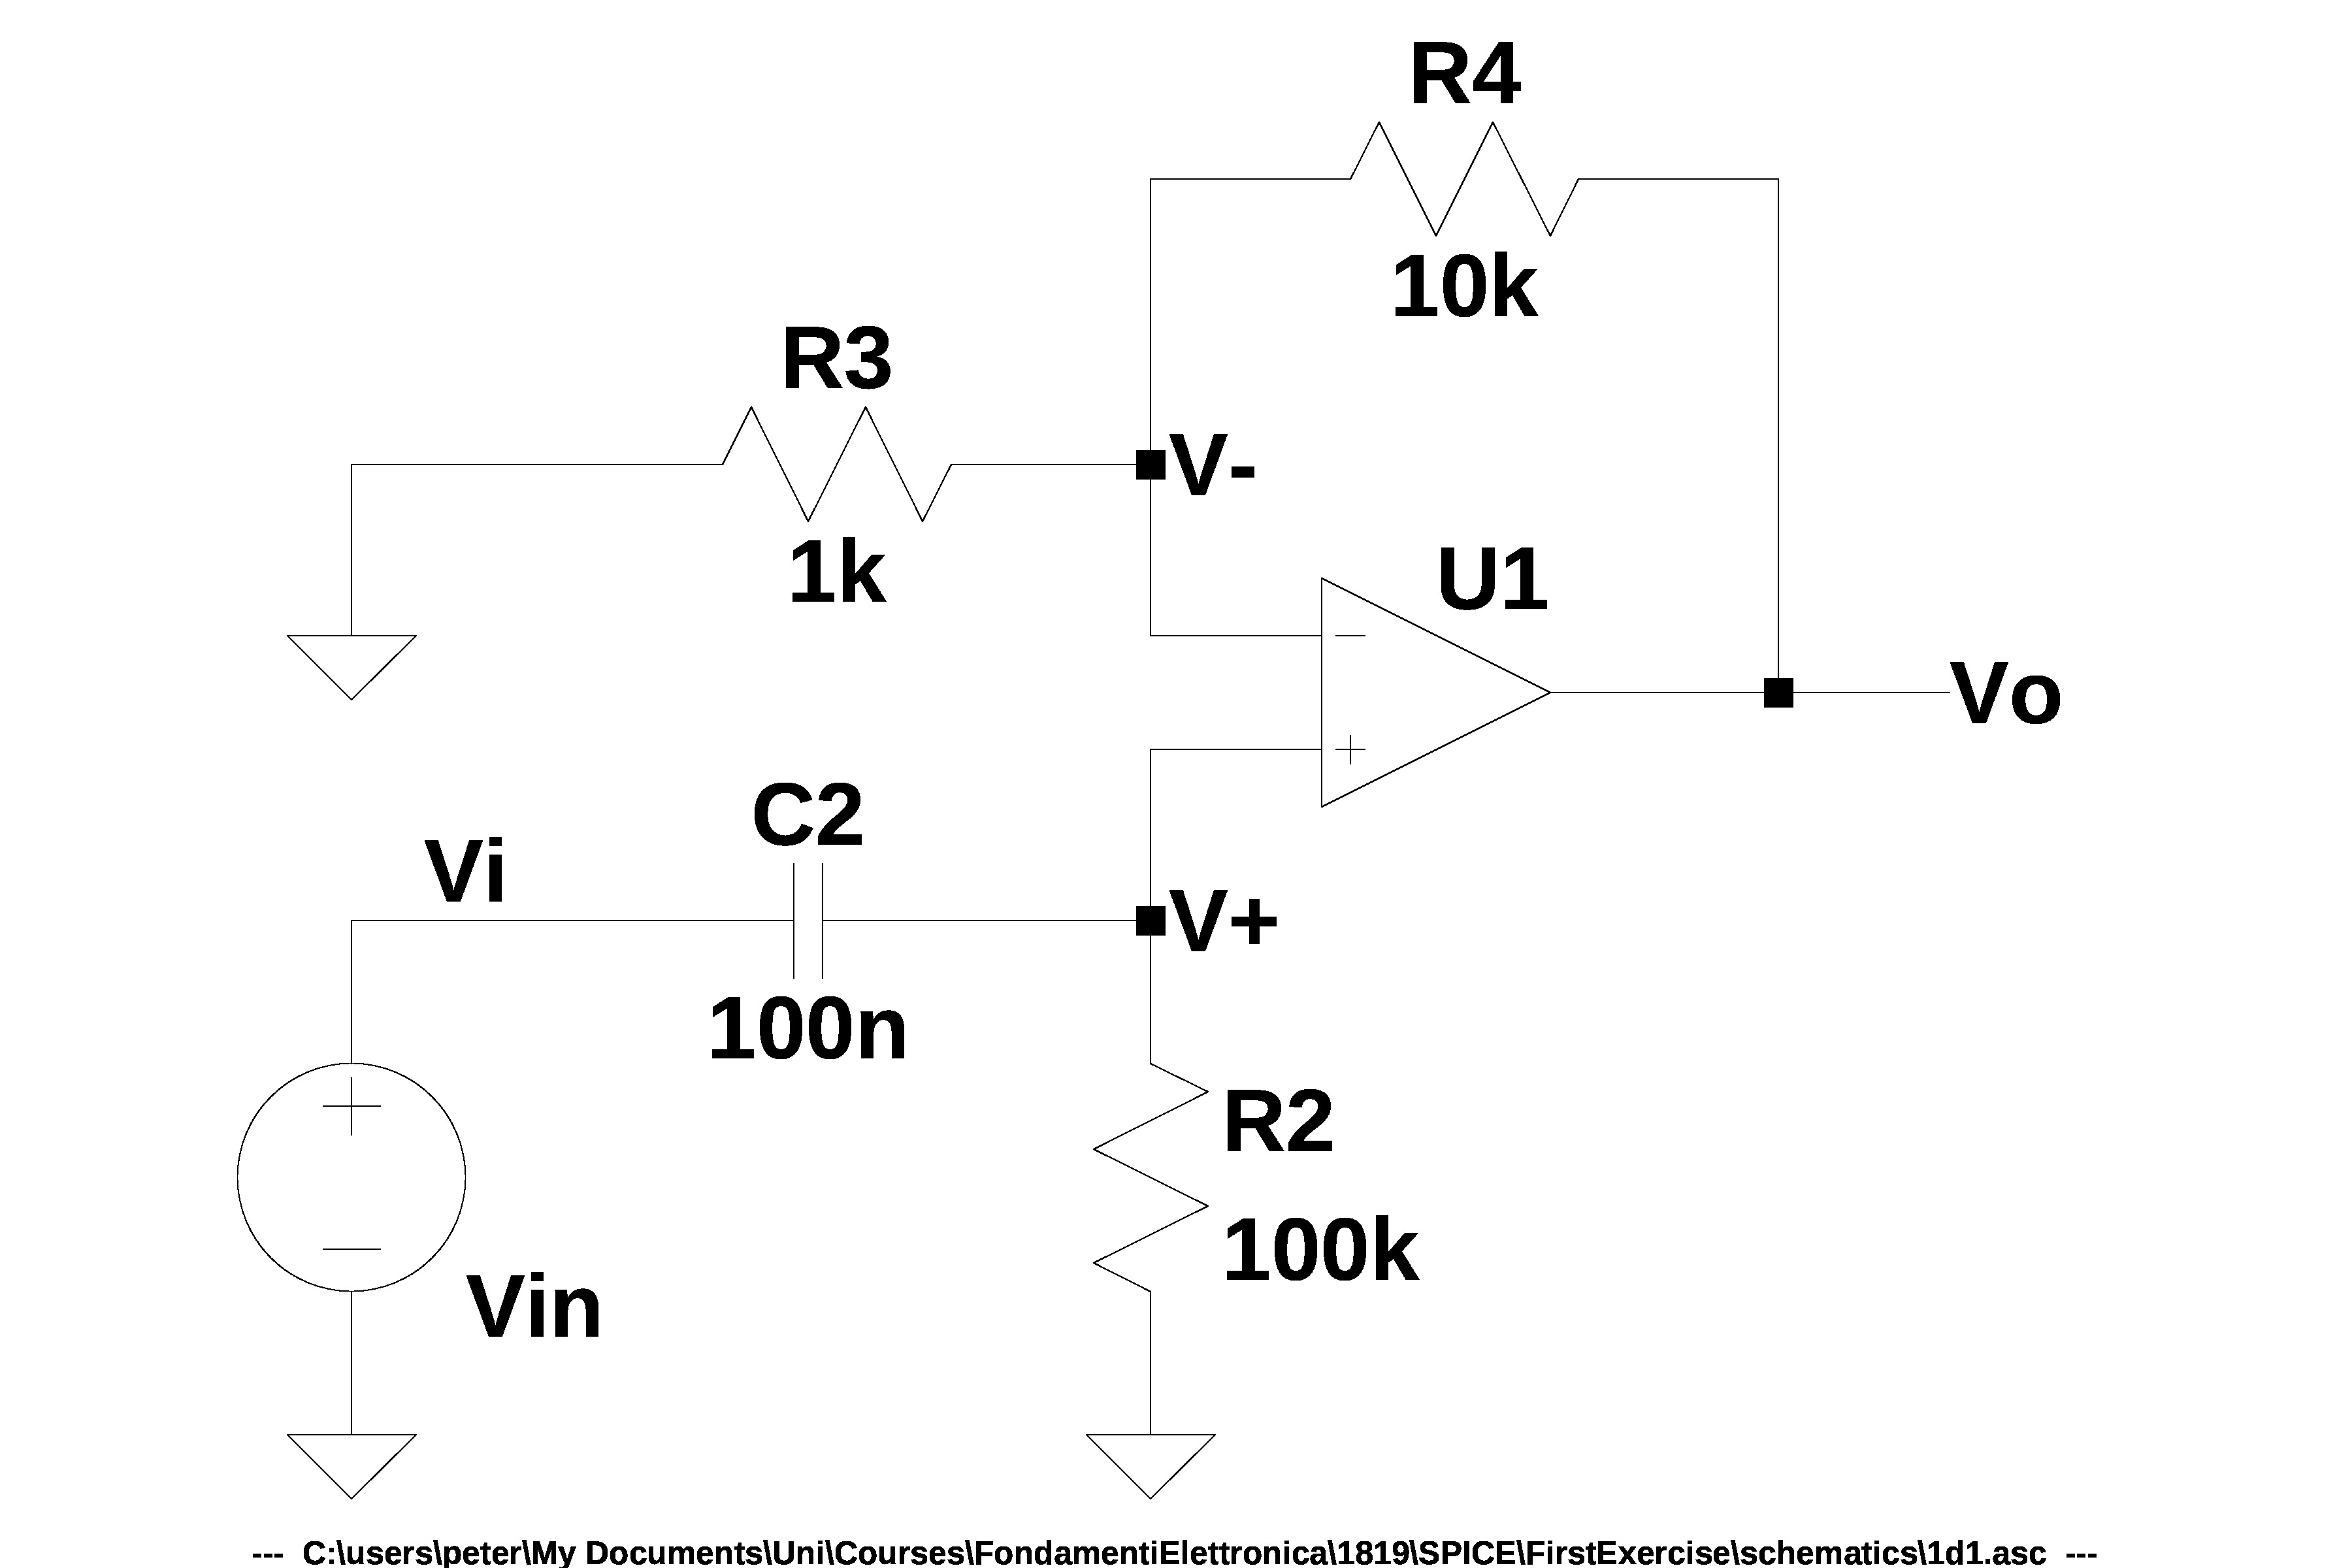
\includegraphics[width=8cm]{schematics/1d1.jpg}
  \caption{Audio amplifier - Ideal op. amp.}
  \label{1d1}
\end{figure}

$$V_+ = V_{in}\frac{R_2\frac{1}{sC_2}}{R_2+\frac{1}{sC_2}} =
V_{in}\frac{R_2\frac{1}{sC_2}}{R_2+\frac{1}{sC_2}}\frac{sC_2}{sC_2} =
V_{in}\frac{R_2}{1+sC_2R_2}$$

$$V_- = V_+$$
$$I_{R_3} = \frac{V_-}{R_3} = \frac{V_+}{R_3} = V_{in}\frac{R_2}{1+sC_2R_2}\frac{1}{R_3}$$
$$I_{R_4} = I_{R_3}$$

$$V_o = V_+ + R_4I_{R_4} =
V_{in}\frac{R_2}{1+sC_2R_2} + V_{in}\frac{R_2}{1+sC_2R_2}\frac{R_4}{R_3} =
V_{in}\frac{R_2}{1+sC_2R_2}\left(1+\frac{R_4}{R_3}\right)$$

$$\frac{V_o}{V_{in}} = \frac{R_2}{1+sC_2R_2}\left(1+\frac{R_4}{R_3}\right) =
\frac{R_2}{1+sC_2R_2}\frac{R_3+R_4}{R_3} = \frac{R_2(R_3+R_4)}{R_3(1+sC_2R_2)} =
\frac{R_2(R_3+R_4)}{R_3}\frac{1}{1+sC_2R_2}$$
$$ K = \frac{R_2(R_3+R_4)}{R_3} = \frac{100 \cdot 10^3(1 \cdot 10^3 + 10 \cdot 10^3)}{1 \cdot 10^3} = 1.1 \cdot 10^6$$

$$ \log_{10}(K) = \log{10}(1.1 \cdot 10^6) \simeq 6$$

$$ \omega_1 = \frac{1}{C_2R_2} =
\frac{1}{100 \cdot 10^{-9} \cdot 100 \cdot 10^3} = 100$$

$$\log_{10} (\omega_1) = \log_{10} (100) = 2$$

\subsection{Waveform}
\begin{figure}[h]
  \centering
  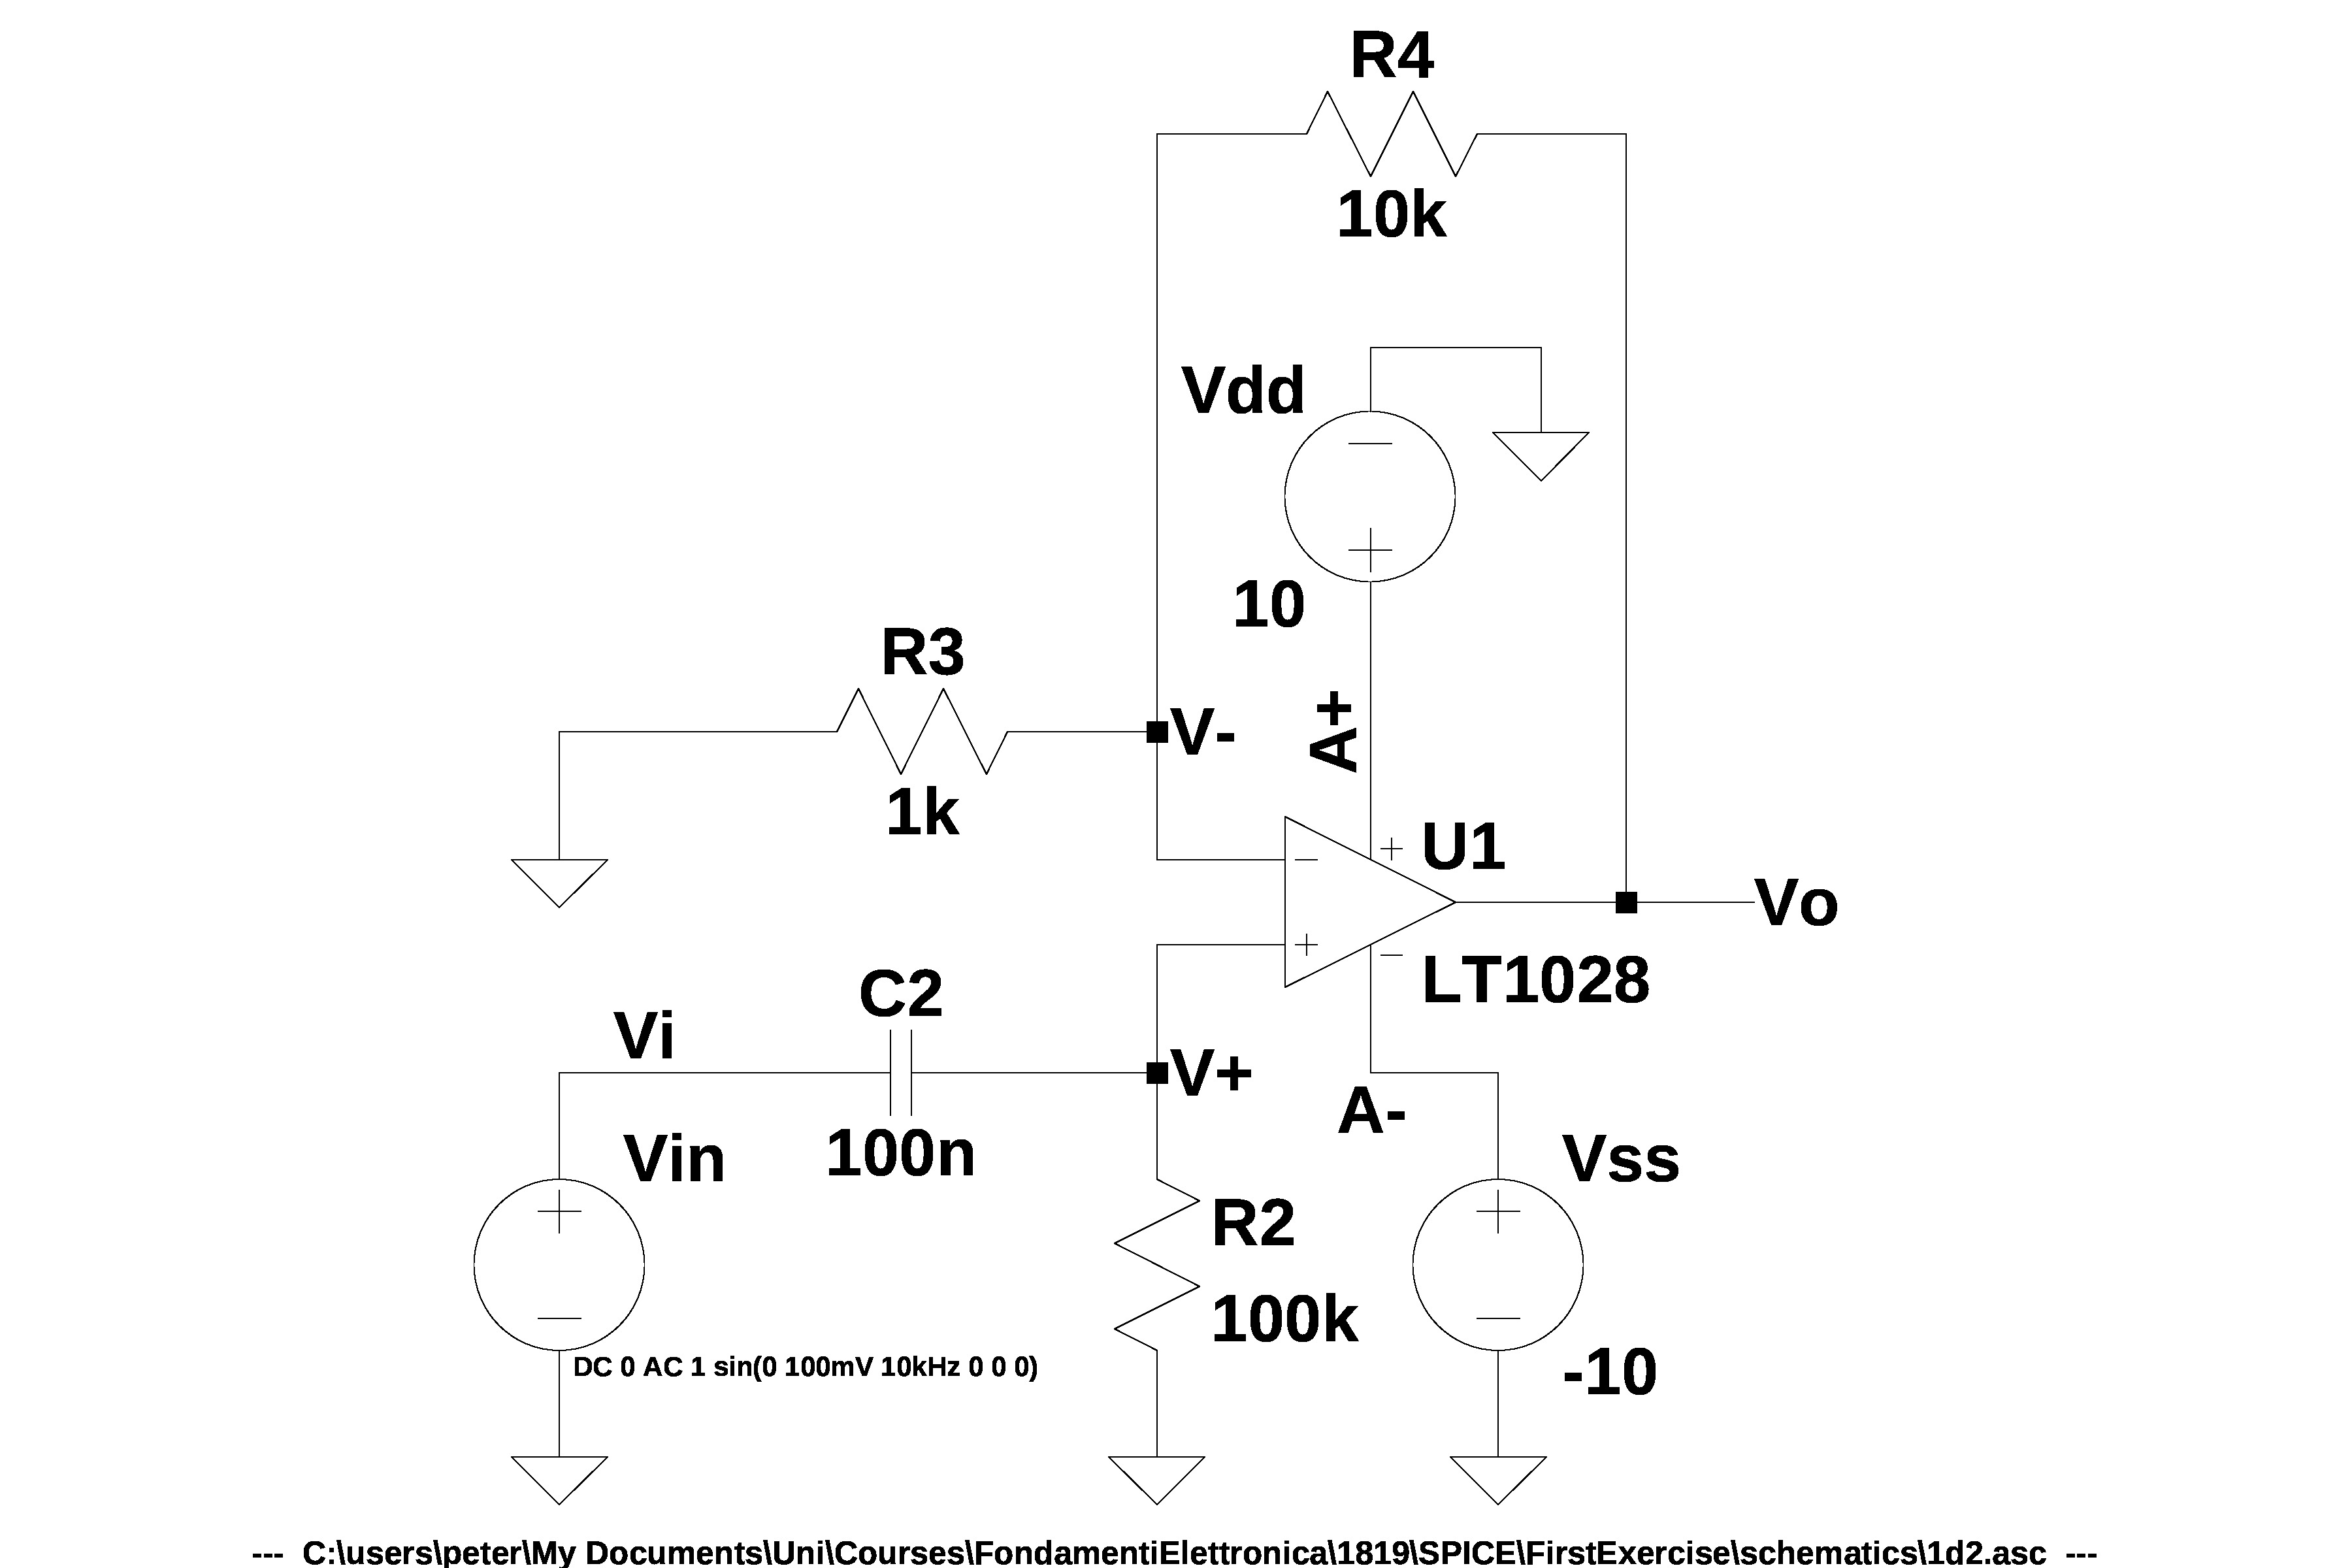
\includegraphics[width=10cm]{schematics/1d2.jpg}
  \caption{Audio amplifier}
  \label{1d2}
\end{figure}

\lstinputlisting{netlist/1d2.cir}

\begin{figure}[h]
  \centering
  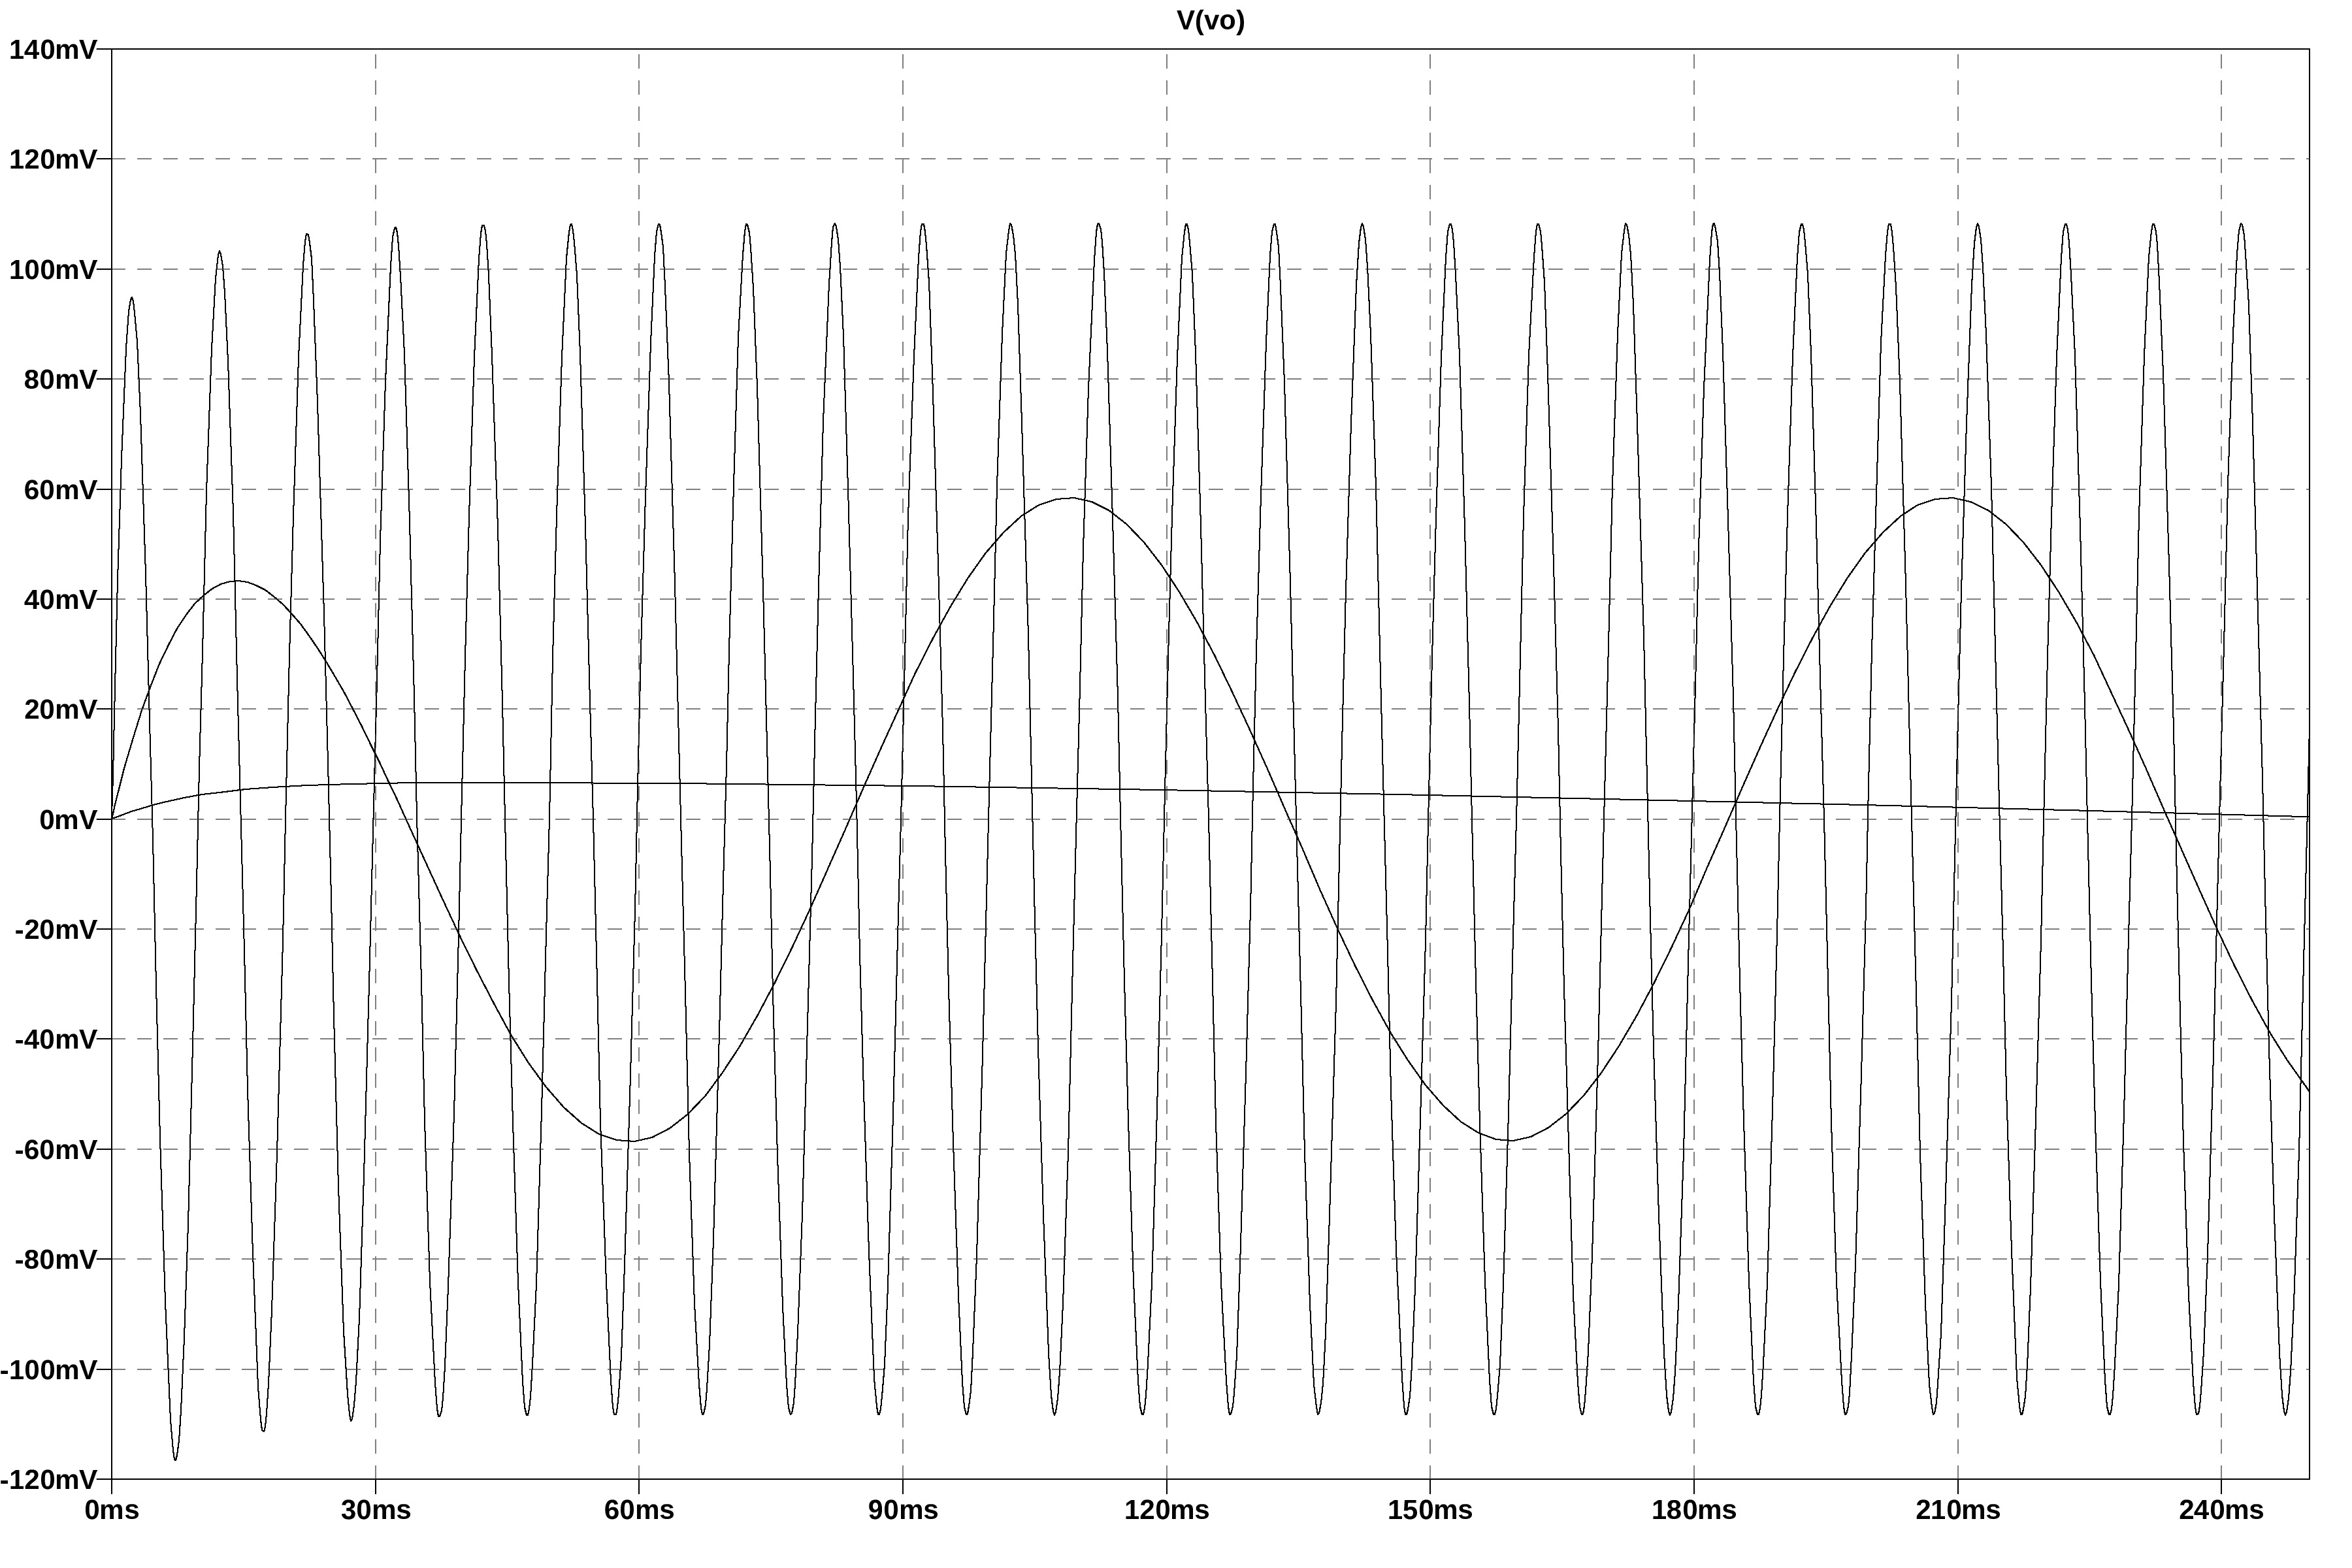
\includegraphics[width=14cm]{graph/1d2.jpg}
  \caption{Voltage output waveform}
  \label{1d2}
\end{figure}

% License
\vspace*{\fill}
\centering
\tiny{This work is licensed under the Creative Commons Attribution-ShareAlike
 4.0 International License. To view a copy of this license, visit
 \href{http://creativecommons.org/licenses/by-sa/4.0/}{http://creativecommons.org/licenses/by-sa/4.0/}
or send a letter to Creative Commons, PO Box 1866, Mountain View, CA 94042,
USA.}

\end{document}
